\documentclass[12pt]{article}
\usepackage{amsmath}
\usepackage{graphicx}
\usepackage{enumerate}
\usepackage[authoryear,numbers]{natbib}
\usepackage{graphicx}
\usepackage[english]{babel}
\usepackage[colorlinks=true, allcolors=blue]{hyperref}
\usepackage{caption}
\usepackage{subcaption}
\usepackage{placeins}
\usepackage{hyperref}
\usepackage{float}
\usepackage[utf8]{inputenc}
\usepackage{hyphenat}
\tolerance=1000
\usepackage{url}
\usepackage{textcomp}
\usepackage{tikz}
\usepackage{hyphenat}
\usepackage{Sweave}
\bibliographystyle{apalike}
\newcommand{\blind}{0}

% DON'T change margins - should be 1 inch all around.
\addtolength{\oddsidemargin}{-.5in}%
\addtolength{\evensidemargin}{-1in}%
\addtolength{\textwidth}{1in}%
\addtolength{\textheight}{1.7in}%
\addtolength{\topmargin}{-1in}%

\begin{document}
\Sconcordance{concordance:si.tex:si.Rnw:1 60 1 1 5 6 1 1 12 1 2 1 1 1 11 1 2 6 1 1 12 %
1 2 1 1 1 11 1 2 1 1 1 11 1 2 1 1 1 11 1 2 6 1 1 12 1 2 1 1 1 11 1 2 6 %
1 1 12 1 2 1 1 1 11 1 2 5 1 1 12 1 2 4 1 1 12 1 2 4 1 1 31 59 1}

\def\spacingset#1{\renewcommand{\baselinestretch}%
{#1}\small\normalsize} \spacingset{1}


\if1\blind
{
  \title{\bf Mechanistic models for panel data: analysis of ecological experiments with four interacting species}
  \author{Author 1\thanks{
    The authors gratefully acknowledge \textit{please remember to list all relevant funding sources in the unblinded version}}\hspace{.2cm}\\
    Department of YYY, University of XXX\\
    and \\
    Author 2 \\
    Department of ZZZ, University of WWW}
  \maketitle
} \fi

\if0\blind
{
  \bigskip
  \bigskip
  \bigskip
  \begin{center}
    {\LARGE\bf Mechanistic models for panel data: analysis of ecological experiments with four interacting species}
\end{center}
  \medskip
} \fi

\bigskip


\section{Simulation}
\label{sec:sim}
\begin{figure}[H]
\centering
\begin{subfigure}[b]{\linewidth}
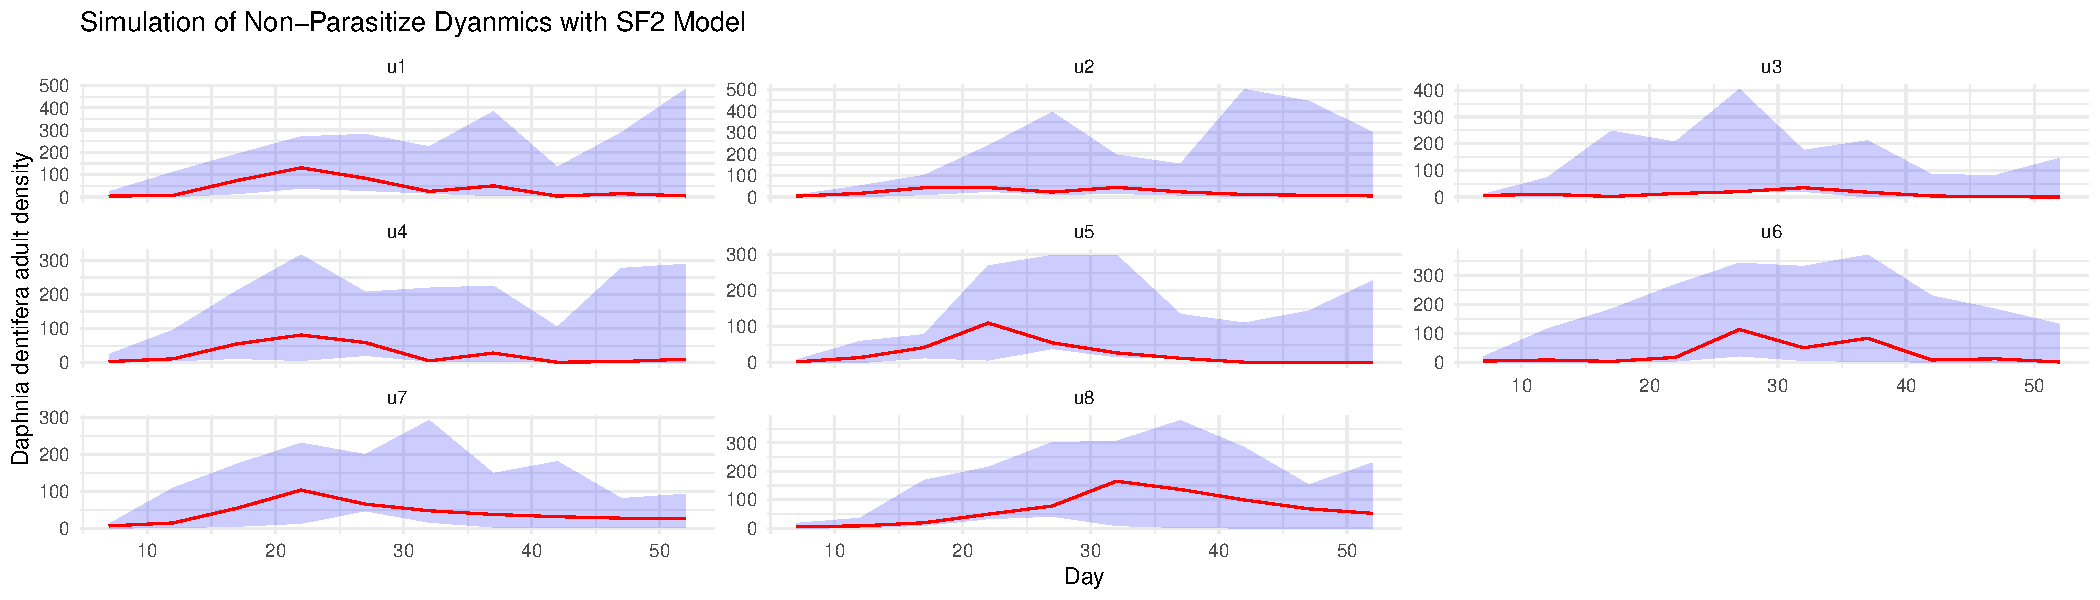
\includegraphics{si-002}
\end{subfigure}
\begin{subfigure}[b]{\linewidth}
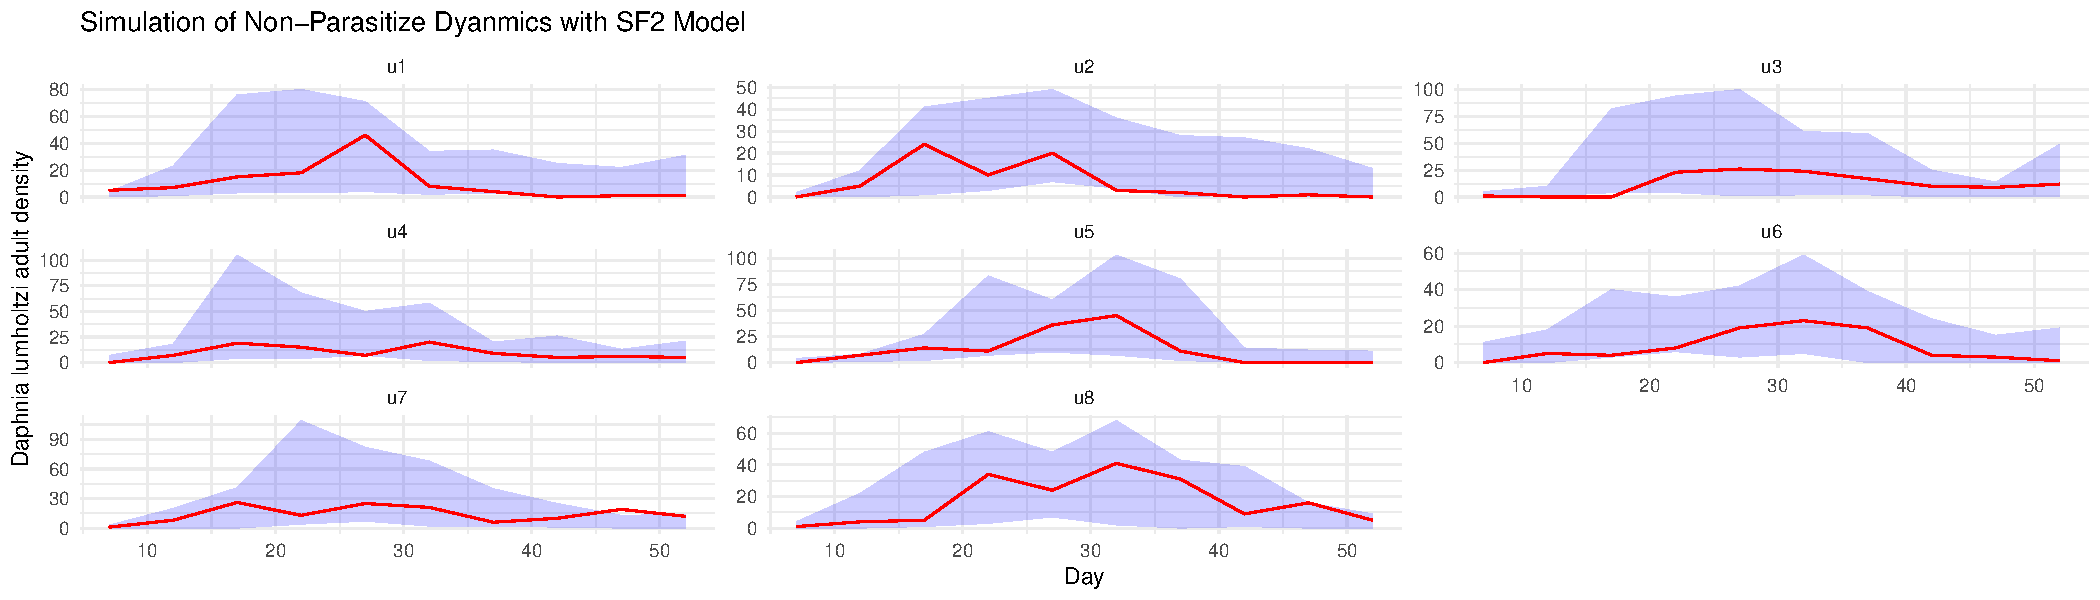
\includegraphics{si-003}
\end{subfigure}%
\caption{Plot of Simulation of Non-Parasitize Dyanmics with SF2 Model. The blue shadow implies the possible range from simulation, while the red line shows the real-world data. The various trail represents different buckets in the experiment}
\end{figure}

\begin{figure}[H]
\centering
\begin{subfigure}[b]{\linewidth}
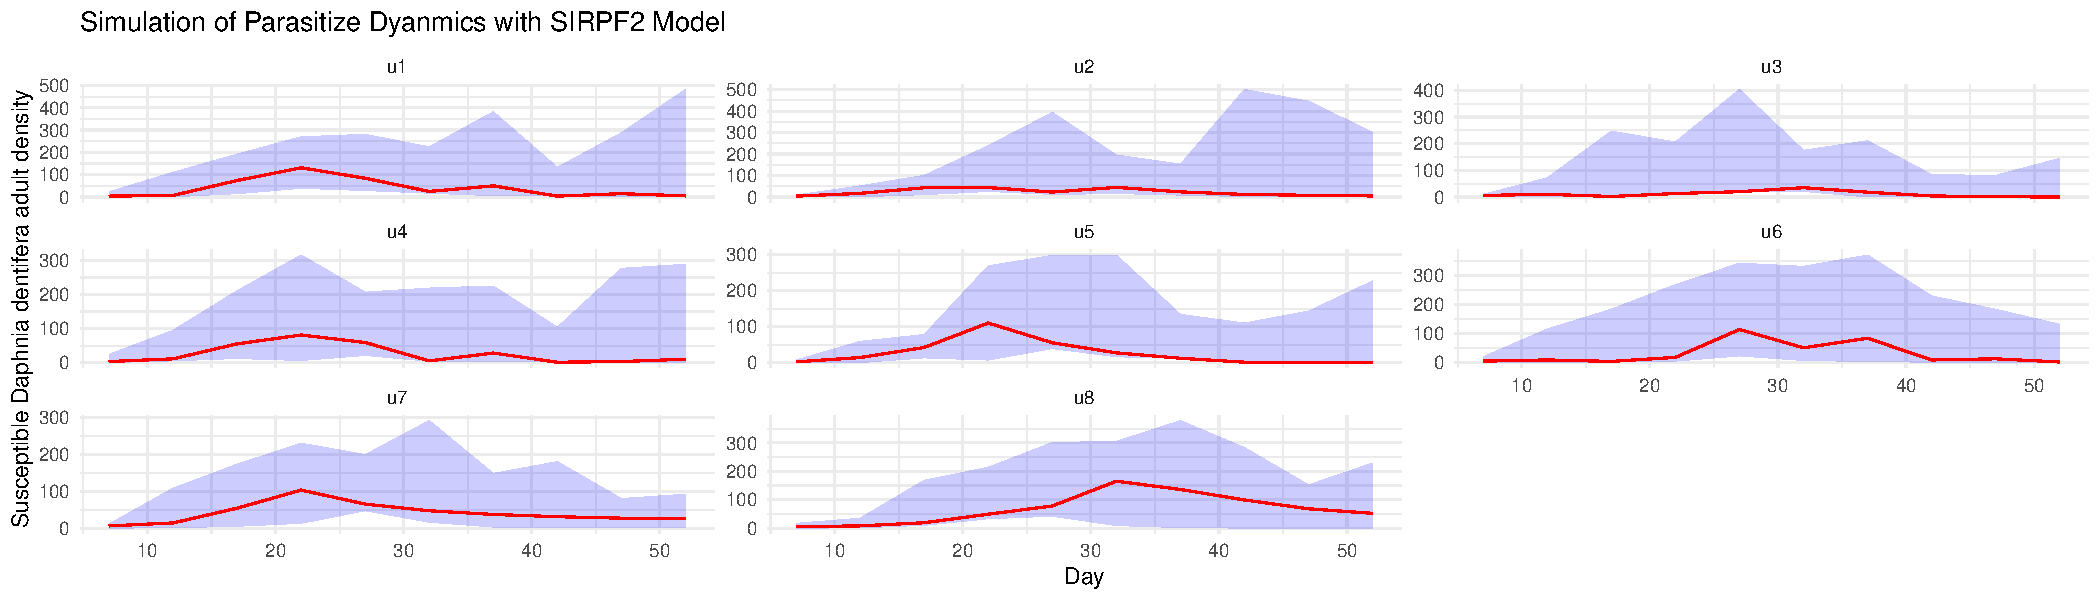
\includegraphics{si-004}
\end{subfigure}
\begin{subfigure}[b]{\linewidth}
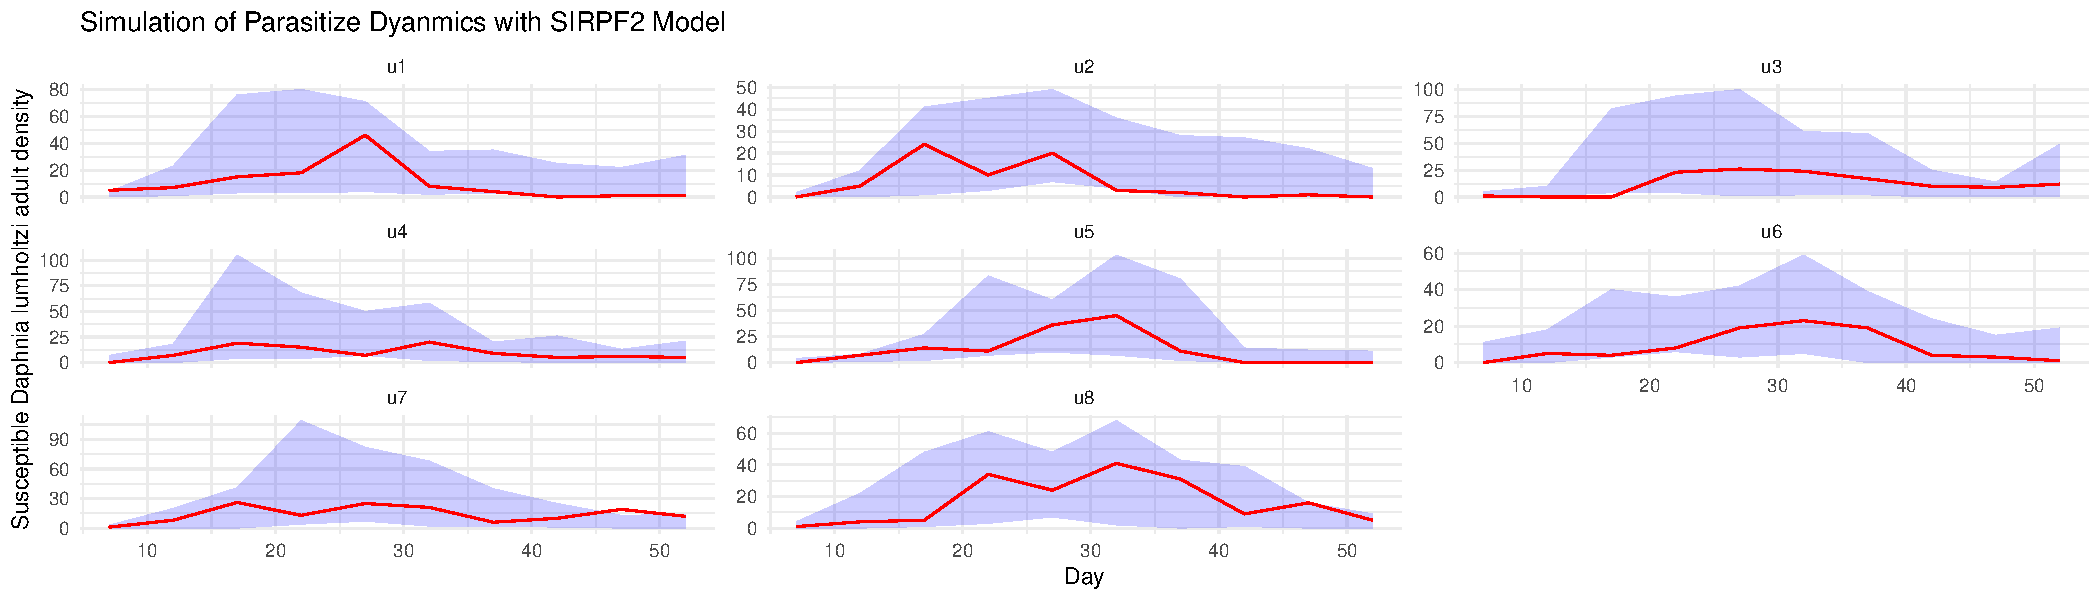
\includegraphics{si-005}
\end{subfigure}
\begin{subfigure}[b]{\linewidth}
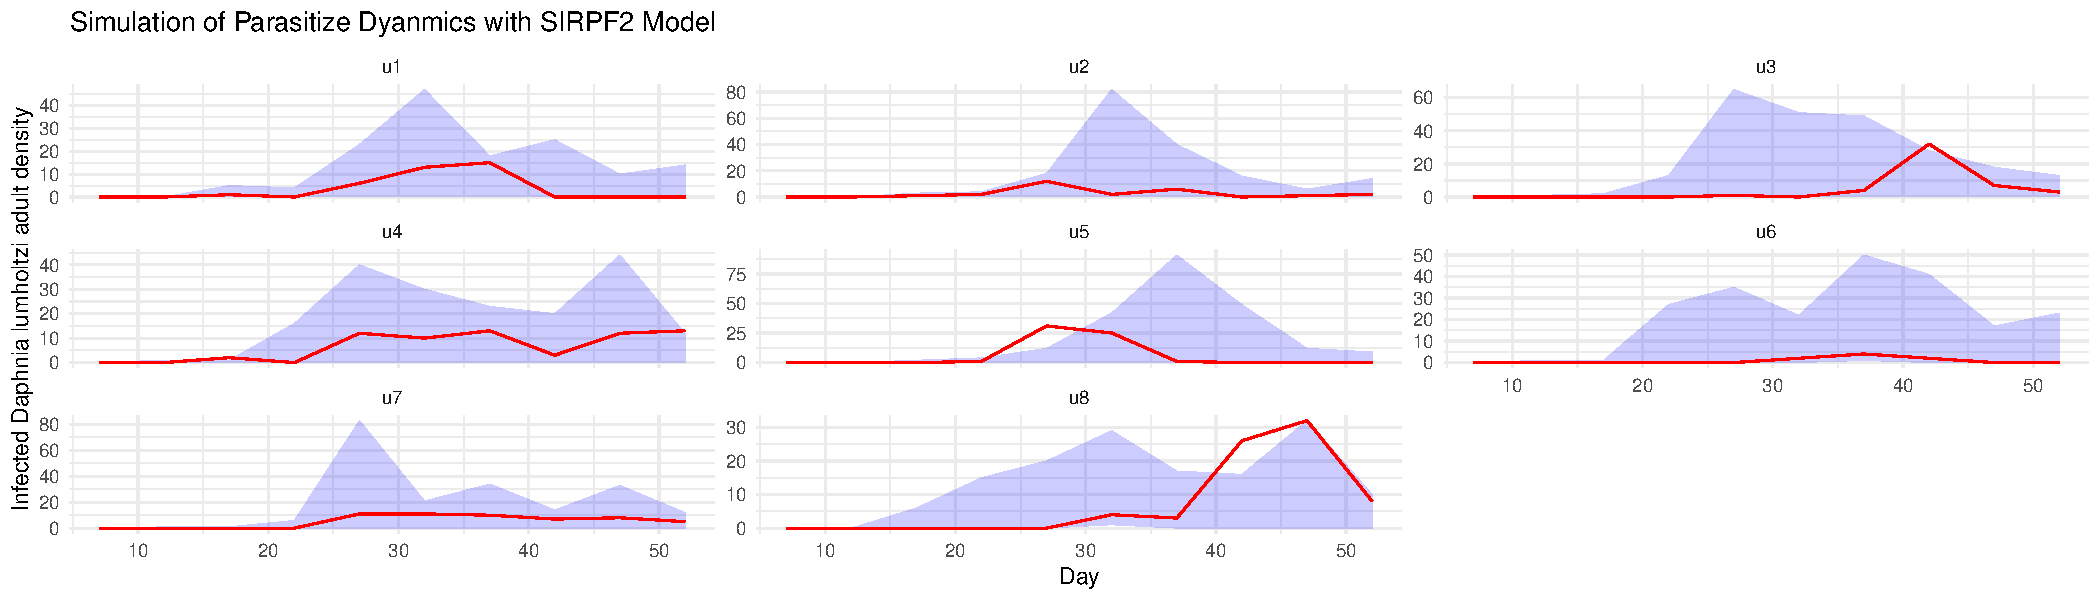
\includegraphics{si-006}
\end{subfigure}
\begin{subfigure}[b]{\linewidth}
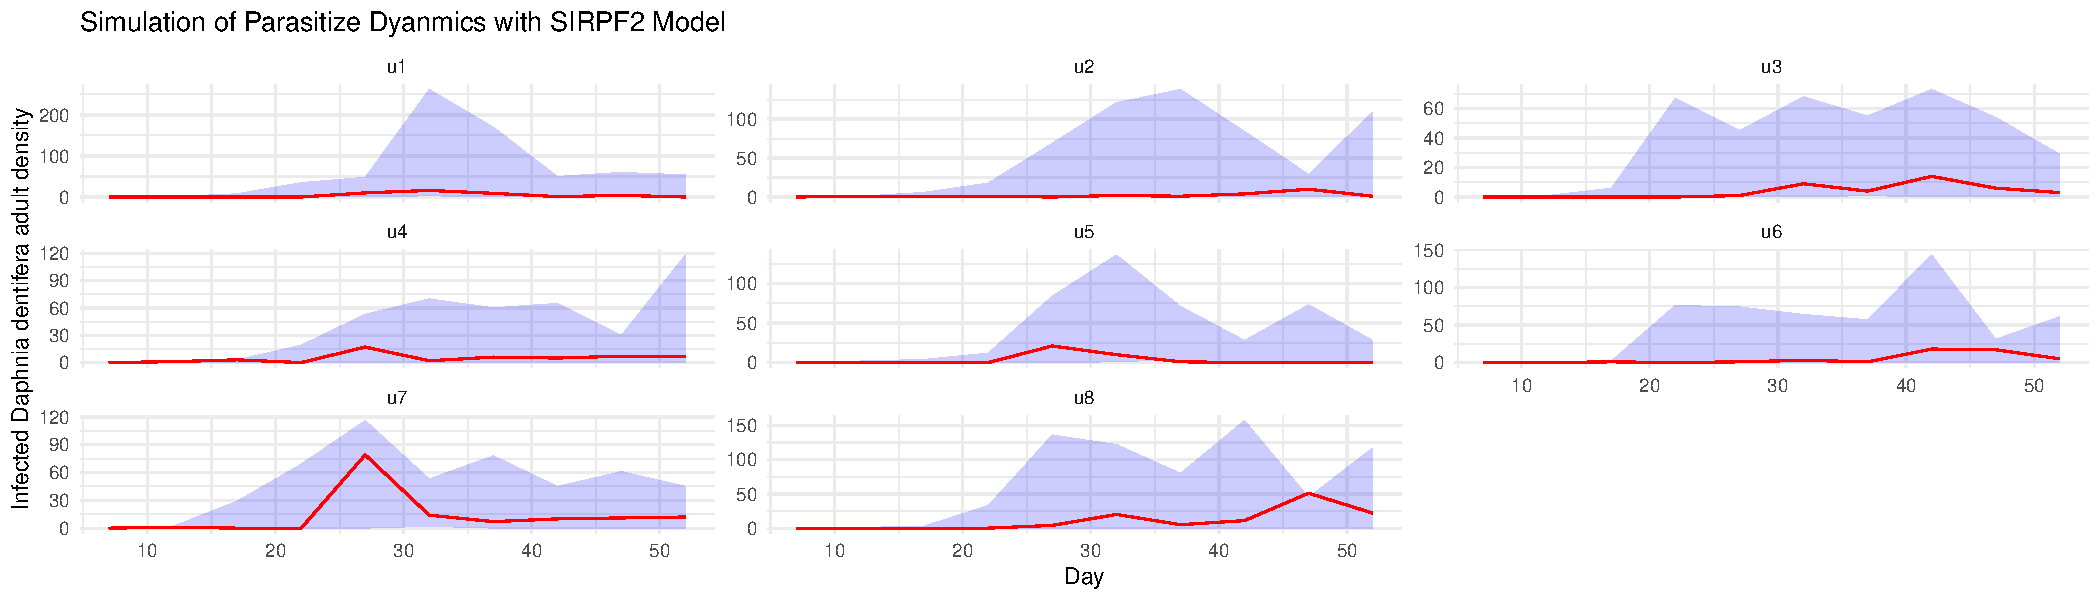
\includegraphics{si-007}
\end{subfigure}%
\caption{Plot of Simulation of Parasitize Dyanmics with SIRPF2 Model. The blue shadow implies the possible range from simulation, while the red line shows the real-world data. The various trail represents different buckets in the experiment}
\end{figure}

\begin{figure}[H]
\centering
\begin{subfigure}[b]{\linewidth}
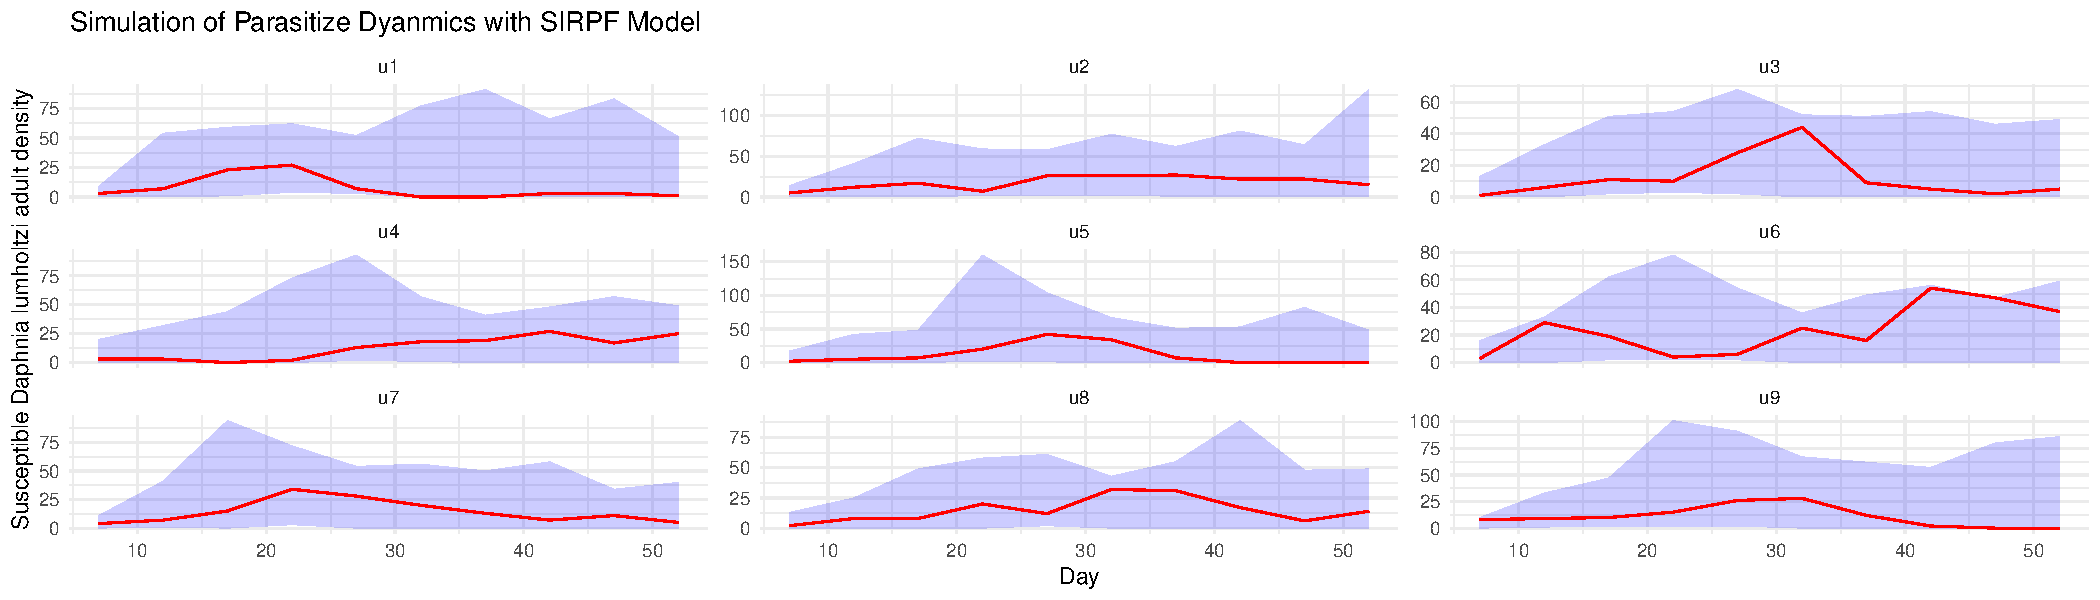
\includegraphics{si-008}
\end{subfigure}
\begin{subfigure}[b]{\linewidth}
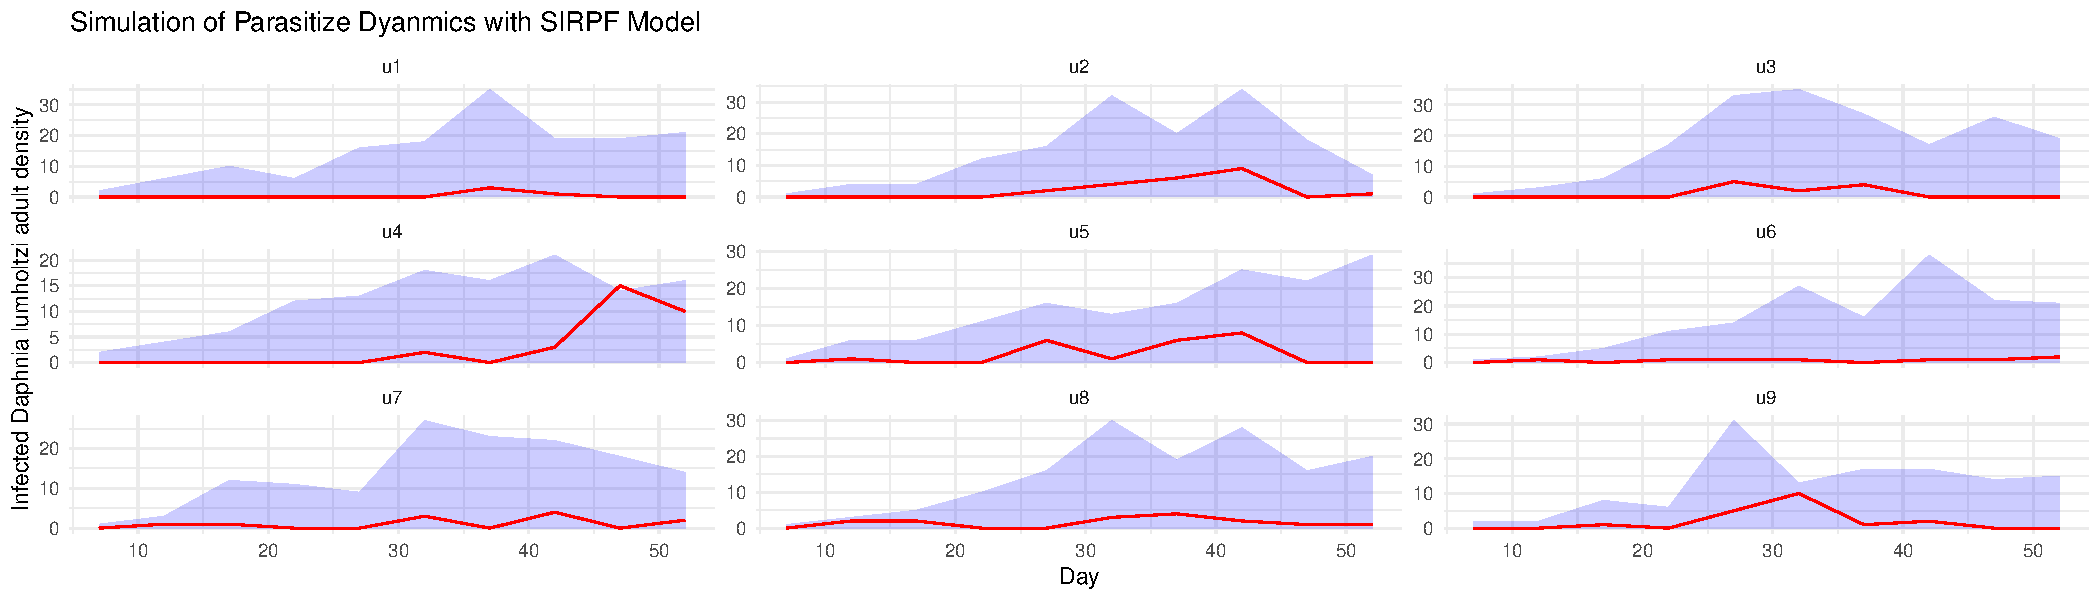
\includegraphics{si-009}
\end{subfigure}%
\caption{Plot of Simulation of Invasive Parasitize Dyanmics with SIRPF Model. The blue shadow implies the possible range from simulation, while the red line shows the real-world data. The various trail represents different buckets in the experiment}
\end{figure}

\begin{figure}[H]
\centering
\begin{subfigure}[b]{\linewidth}
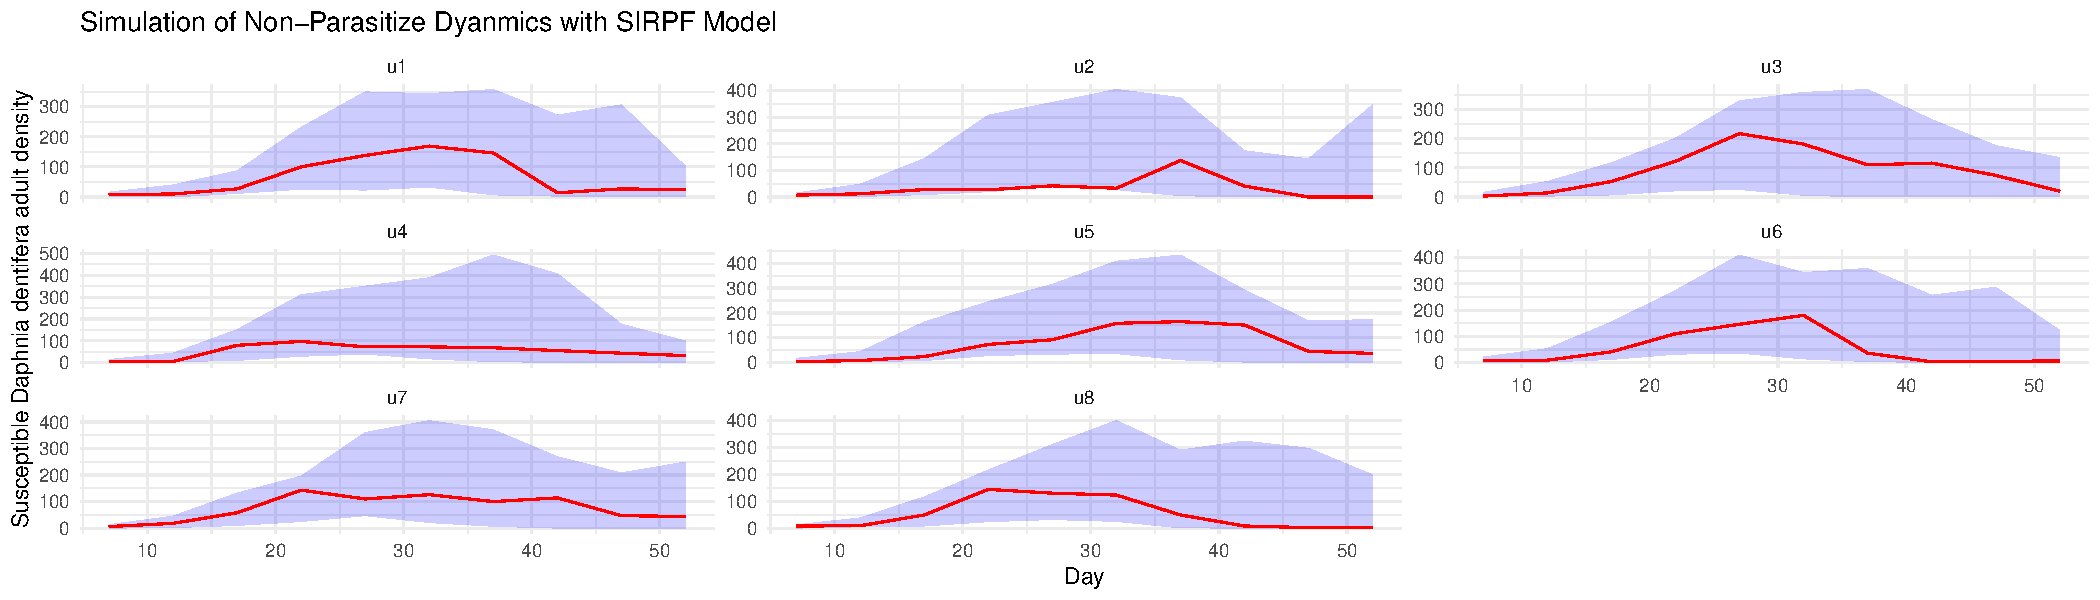
\includegraphics{si-010}
\end{subfigure}
\begin{subfigure}[b]{\linewidth}
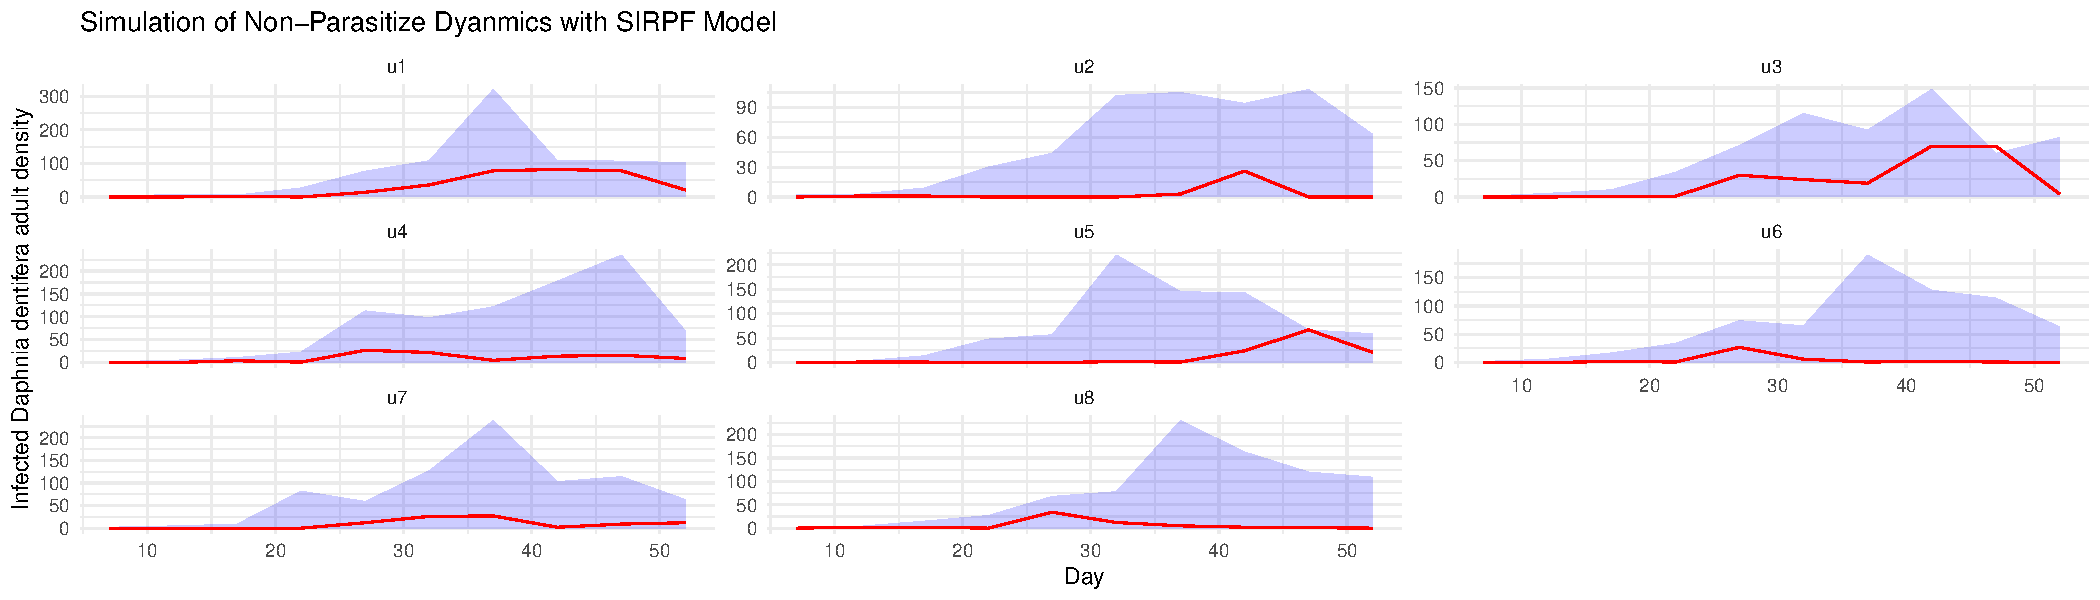
\includegraphics{si-011}
\end{subfigure}%
\caption{Plot of Simulation of Native Parasitize Dyanmics with SIRPF Model. The blue shadow implies the possible range from simulation, while the red line shows the real-world data. The various trail represents different buckets in the experiment}
\end{figure}

\begin{figure}[H]
\centering
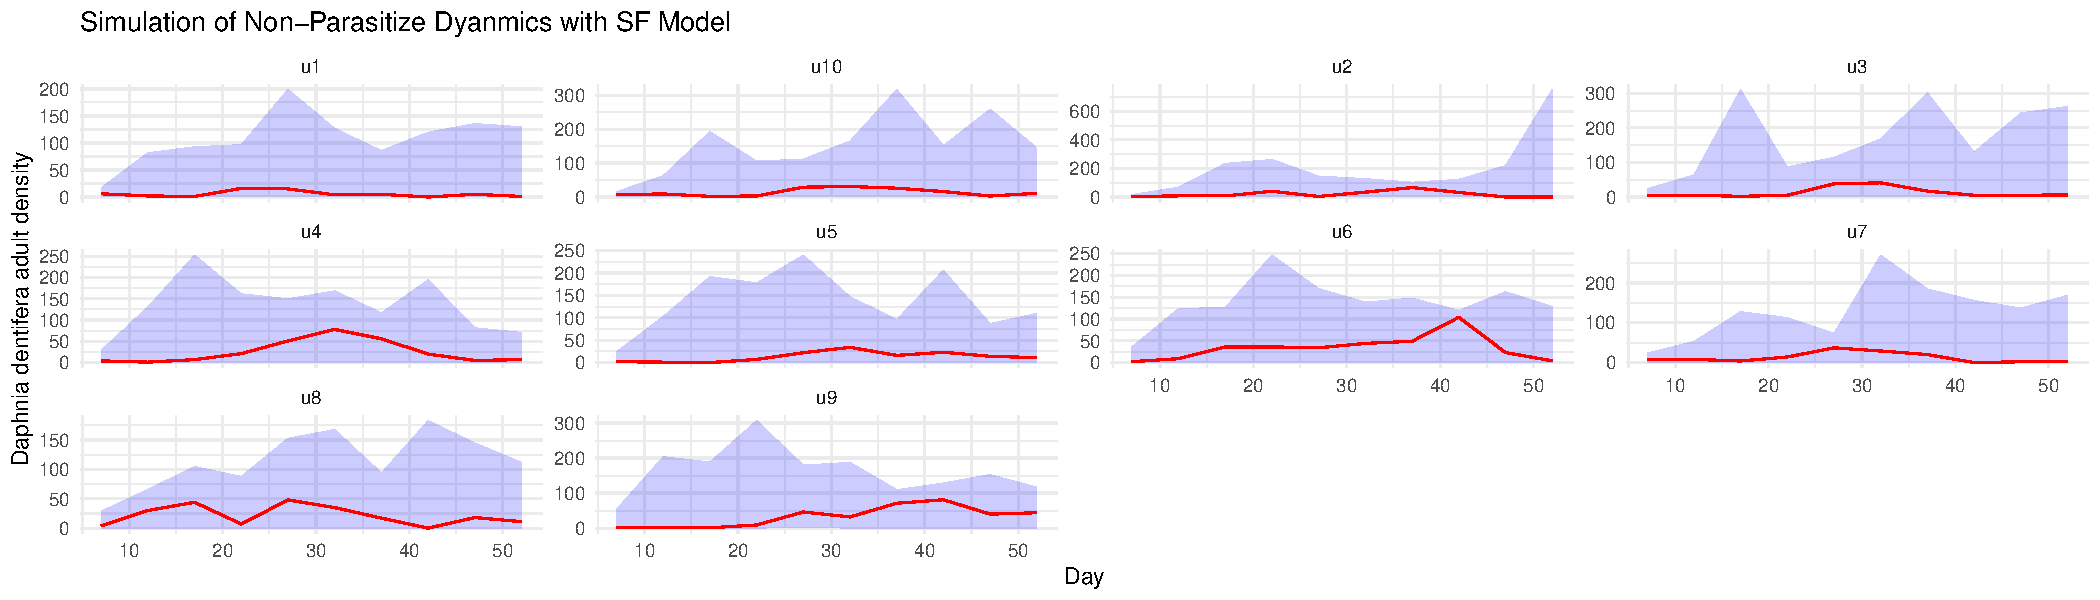
\includegraphics{si-012}
\caption{Plot of Simulation of Native Non-Parasitize Dyanmics with SF Model. The blue shadow implies the possible range from simulation, while the red line shows the real-world data. The various trail represents different buckets in the experiment}
\end{figure}

\begin{figure}[H]
\centering
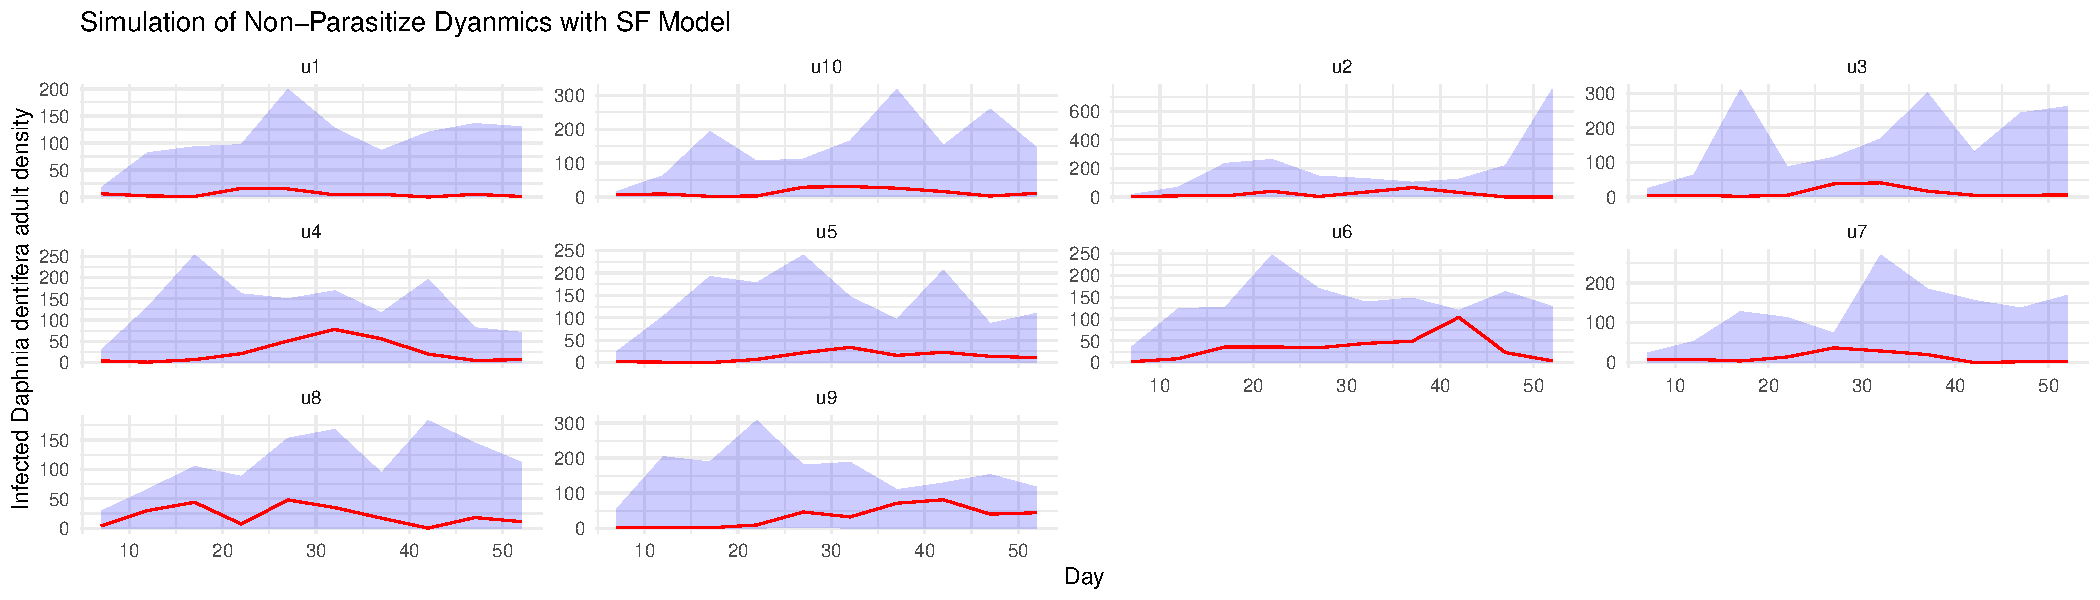
\includegraphics{si-013}
\caption{Plot of Simulation of Invsaive Non-Parasitize Dyanmics with SF Model. The blue shadow implies the possible range from simulation, while the red line shows the real-world data. The various trail represents different buckets in the experiment}
\end{figure}

\newpage
\section{Tables}
\renewcommand{\arraystretch}{0.5}
\begin{table}[H]
\centering
\resizebox{\textwidth}{!}{\begin{tabular}{||c|c |c|c||}
 \hline
Parameter & Definition &Unit\\[0.5ex]
\hline\hline
$S_j$ & Susceptible host density for species $j$  &$individuals \cdot L ^{-1}$ & Variable\\
$I_j$ & Infected host density for species $j$ & $ individuals \cdot L ^{-1}$&Variable\\
$F$& Alga density& $10^5 cells \cdot L ^{-1}$&Variable\\
$P$ & Spore density & $10^3 spores \cdot L ^{-1}$&Variable\\
$K_F$ & Alga carrying capacity&$10^5 cells \cdot L ^{-1} $& 0.092\\
$r_n$ & Native growth rate &$10^{-5} \cdot cells^{-1} \cdot day^{-1}$& 0.23\\
$r_i$ & Invasive growth rate &$10^{-5} \cdot cells^{-1} \cdot day^{-1}$&0.23\\
$\theta_{I_n}$ & Native infected host mortality rate&$ day^{-1}$&0.66 \\
$\theta_{I_i}$ & Invasive infected host mortality rate&$ day^{-1}$&0.37 \\
$\theta_{S_i}$ & Invasive susceptible host mortality rate&$ day^{-1}$&0.086 \\
$\theta_{S_n}$ & Native susceptible host mortality rate&$ day^{-1}$& 0.098 \\
$\theta_{P}$ & Spore degradation rate&$ day^{-1}$&0.015 \\
$p_n$ &Native probability of infection per spore &$10^{-3} \cdot individuals \cdot spore^{-1} $& 0.92\\
$p_i$ & Invasive probability of infection per spore&$10^{-3} \cdot individuals \cdot spore^{-1} $& 0.98\\
$f_{S_n}$ & Native susceptible host filtering rate&$L \cdot day^{-1} \cdot individuals^{-1} $& 0.00027\\
$f_{S_i}$ & Invasive susceptible host filtering rate&$L \cdot day^{-1} \cdot individuals^{-1} $& 0.00027\\
$f_{I_n}$ & Native infected host filtering rate&$L \cdot day^{-1} \cdot individuals^{-1} $& 0.0018\\
$f_{I_i}$ & Invasive infected host filtering rate&$L \cdot day^{-1} \cdot individuals^{-1} $& 0.000067 \\
$\delta$ & Sampling rate&$day ^{-1} $& constant = 0.013\\
$\alpha$ & Alga maximum exponential growth rate&$day ^{-1} $ & 0.011\\
$\gamma_n$ & Native host consumption rate&$L \cdot inidviduals^{-1} \cdot day ^{-1} $ & 0.000030\\
$\gamma_i$ & Invsaive host consumption rate&$L \cdot inidviduals^{-1} \cdot day ^{-1} $ & 0.00067\\
$\mu$ & Alag refilling rate&$10^5 cells \cdot L ^{-1} \cdot day^{-1}$ & constant = 0.37\\
$\xi$ &Reduction in infected host reproduction and consumption& $Unitless$ & 0.00041\\
$\beta_i$ & Spores produced per infected invasive species&$10^3 \cdot spores \cdot individuals^{-1} $ &3.8\\
$\beta_n$ & Spores produced per infected native species&$10^3 \cdot spores \cdot individuals^{-1} $ &3.2\\
$\sigma_{S_n}$ & Standard deviation of brownian motion of susceptible native&$\sqrt{individual \cdot t^{-1}}$ & 0.061\\
$\sigma_{S_i}$ & Standard deviation of brownian motion of susceptible invasive &$\sqrt{individual \cdot t^{-1}}$ & 0.11\\
$\sigma_{I_n}$ & Standard deviation of brownian motion of infected native&$\sqrt{individual \cdot t^{-1}}$ & 0.45\\
$\sigma_{I_i}$ & Standard deviation of brownian motion of infected invasive&$\sqrt{individual \cdot t^{-1}}$ & 0.0018\\
$\sigma_{F}$ & Standard deviation of brownian motion of alga&$\sqrt{individual \cdot t^{-1}}$ & 0.29\\
$\sigma_{P}$ &Standard deviation of brownian motion of parasite &$\sqrt{individual \cdot t^{-1}}$ & 0.20\\
$k_{S_n}$ & Overdispersion parameter& $Unitless$ &4.5\\
$k_{S_i}$ &Overdispersion parameter &$Unitless$ &5.4\\
$k_{I_n}$ &Overdispersion parameter &$Unitless$ &1.4\\
$k_{I_i}$ & Overdispersion parameter&$Unitless$ &1.2\\[1ex]
 \hline
\end{tabular}}
\caption{This table shows the units of the parameters of competition SIRPF2 model}
\label{Table:1}
\end{table}
\renewcommand{\arraystretch}{1}









\bibliography{reference}
\end{document}
